\section{Experiment}
\label{sec:experiment}
In this section, we will introduce our experiment setup and results.
%We will show the advantages of our two-step framework over the end-to-end pre-trained model and other strong baselines on three datasets.
%\textcolor{green}{Not only experiment setup?}



\begin{comment}
\KZ{The following descriptions of the 3 datasets are too verbose.
Simplify each into one or two sentences and put into \tabref{tab:statitics-datasets}.}
\begin{itemize}
%\item Question Rewriting in Conversational Context (\textbf{QReCC}) \citep{anantha-etal-2021-open}. The authors built it on questions from TREC CAsT \citep{DBLP:journals/corr/abs-2003-13624}, QuAC \citep{choi-etal-2018-quac} and Google Natural Questions \citep{kwiatkowski-etal-2019-natural}. Its task is to find answers to conversational questions within a collection of 10M web pages split into 54M passages.

\item Context Abstraction: Necessary Additional Rewritten Discourse (\textbf{CANARD}) \citep{elgohary-etal-2019-unpack}. The authors crowdsource context-independent paraphrases of QUAC \citep{choi-etal-2018-quac} questions and use the paraphrases to train and evaluate question-in-context rewriting. The first sentence of the multi-turn dialogue is usually a news title or the name of a person. Then two people will 
%ask and answer 
talk around the 
%content
context. 
%and 
The rewriting of the current turn of question will be given at the end.

\item Contextual Query Rewrite (\textbf{CQR}) \citep{DBLP:journals/corr/abs-1903-11783}. One task-oriented multi-turn dialogue dataset, the dialogues in which take place between human users and intelligent agents. Users will ask the intelligent agent to 
%meet their needs 
answer specific questions such as driving or shopping. The user's unclear requirements will be completed as the ground truth.

\item Multi-domain Coreference (\textbf{MuDoCo}) \citep{martin-etal-2020-mudoco}. The dataset contains authored dialogs between a ficional user and system, where the user asks the system to perform extensive tasks within multiple domains, as well as switch across a set of 6 task domains (calling, messaging, reminders, weather, news, and music).

%and CamRest676 dataset from the restaurant domain annotated with coreference and ellipsis (\textbf{CamRest}) \citep{quan-etal-2019-gecor}.



\end{itemize}

\end{comment}


\begin{table}[th]
\setlength\tabcolsep{3pt}
\centering
\scriptsize
%\small
%\begin{tabular}{lrrrr}
\resizebox{\linewidth}{!}{\begin{tabular}{lccccc}
%\hline
\toprule
 &    \textbf{MuDoCo} & \textbf{CQR} & \textbf{REWRITE} & \textbf{RES} & \textbf{CANARD} \\ \midrule
%Desc. &	\tabincell{l}{Teacher and \\student talking \\about a news title \\or a person.}	&	\tabincell{l}{Task-oriented \\dialogue between a \\user and an agent.}	&	\tabincell{l}{Daily conversation \\of six domains.}	\\ \midrule
Train & 2.39k  & 0.52k & 16.00k & 193.77k &   16.88k\\
Dev  & 0.29k & 0.06k & 2.00k & 5.10k &  1.79k\\
Test &  0.30k  & 0.06k & 2.00k & 5.10k &  2.96k\\
Ave Len    & 73.43  & 143.70 & 36.85 & 68.38 &  429.77\\
\% RW & 26.68 & 98.38 &  99.98 & 60.00 & 92.91\\
\bottomrule
\end{tabular}}
\caption{Descriptions of the datasets. ``Ave Len'' means the average length of context. ``\% RW'' denotes 
the percentage of samples whose current utterance is actually rewritten.}
%\KZ{This is not clear what it is: is percentage of dialogue instance that is rewritten or
%percentage of utterances that is rewritten? Give a formula if u can't say it clearly: ``/% RW'' means the occurrence rate of rewriting.}
\label{tab:statitics-datasets}
\end{table}

%\KZ{The first few subsections on experimental setup are a bit too
%verbose. They take up more than one page. Can you cut them down and
%spend your text on the more important parts which are the analysis of the
%results?}
\subsection{Datasets}
%\KZ{Cite the three datasets in the text below.}
We tested the baseline and our framework on 3 public datasets in English and 2 in Chinese.
The statistics are shown in \tabref{tab:statitics-datasets}. The examples are shown in Appendix.

 
%the highest difficulty. 
%Our research is mainly conducted on CANARD. 
\textbf{MuDoCo} \citep{martin-etal-2020-mudoco} 
has a lower rewriting rate, which makes the rule-based method less accurate in predicting the locations to be rewritten.
% CANARD is a question and answer dialogue dataset between two people around a topic.
%The sentence pattern is complex, the understanding is difficult, and the rewriting degree is higher. 
\textbf{CQR} \citep{DBLP:journals/corr/abs-1903-11783} contains imperative dialogues in life (between people or between people and intelligent agents). The sentence patterns are relatively simple, fixed and easy to understand.
\textbf{REWRITE} \citep{DBLP:conf/acl/SuSZSHNZ19} is a Chinese dataset, each dialogue of which contains 3 turns. It is collected from several popular Chinese social media platforms. The task is to complete the last turn.
\textbf{RES} (Restoration-200k) \citep{DBLP:conf/emnlp/PanBWZL19} is a large-scale Chinese dataset in which 200K multi-turn conversations are collected and manually labeled with the explicit relations between an utterance and its context. Each dialogue is longer than REWRITE.
\textbf{CANARD} \citep{elgohary-etal-2019-unpack} contains a series of English dialogues about a certain topic or person organized in the form of QA. It has the largest size and the longest context length.
%and is the most difficult.
The sentence pattern in CANARD is complex, the understanding is difficult, and the rewriting degree is high.
%As CANARD is the most challenging dataset among the three,
%our research is mainly conducted on CANARD.

\begin{table*}[ht!]
%\setlength\tabcolsep{3pt}
\centering
\scriptsize
%\small
%\begin{tabular}{lrrrrrrr}
%\resizebox{\linewidth}{!}{
\begin{tabular}{l|ccc|ccc|ccc}
%\hline
\toprule
\textbf{Datasets} & \multicolumn{3}{c|}{CQR} &\multicolumn{3}{c|}{MuDoCo} &\multicolumn{3}{c}{CANARD} \\ \midrule
\textbf{Methods}&    \textbf{F}$_{1/2}$ & \textbf{BLEU}$_{1/2}$ & \textbf{ROUGE}$_{1/2/L}$&    \textbf{F}$_{1/2}$ & \textbf{BLEU}$_{1/2}$ & \textbf{ROUGE}$_{1/2/L}$ &    \textbf{F}$_{1/2}$ & \textbf{BLEU}$_{1/2}$ & \textbf{ROUGE}$_{1/2/L}$  \\ \midrule
HCT    & 58.6/32.3 & 64.2/52.9  & 67.8/47.3/65.6 & 56.1/49.2 & 93.0/90.7  & 94.9/87.8/94.9  & 33.9/28.4 & 67.9/61.7  & 80.1/66.5/79.5 \\
RUN    & 54.0/29.5 & 63.1/51.9  & 67.3/45.1/64.3 & 44.8/32.0 & 93.0/90.2  & 94.4/85.4/94.3  & 43.8/30.5 & 70.1/62.2  & 80.5/62.9/79.0 \\
RAST    & 60.9/33.7 & 65.4/53.8  & 69.0/50.6/67.7  & 58.9/50.7 & 92.4/89.9  & 94.0/84.7/93.8 & 44.8/30.8 & 70.5/62.9  & 80.6/63.8/79.4  \\
T5-small & 80.8/72.3 & 62.3/59.9 & 84.3/76.8/83.0  & 62.4/56.7 & 87.5/79.4 & 95.0/88.4/94.9  & 51.5/40.4 & 70.4/64.1  & 80.2/66.6/78.1 \\
BART-base & 79.4/71.7 & 61.5/57.4 & 82.0/74.4/81.9  & 60.8/54.9 & 85.6/78.4 & 93.9/87.3/93.7  & 52.3/41.2 & 68.8/62.6  & 78.9/65.5/77.0 \\
Ours-rule  & 65.0/57.7 & 69.5/65.2 & 72.3/60.3/69.7  & 60.4/47.4 & 83.0/78.3  & 92.3/80.6/92.0 & 51.8/40.5 & 70.9/64.6  & 80.8/67.0/79.0  \\
Ours-T5   & \textbf{87.5}/\textbf{80.3} & \textbf{88.6}/\textbf{85.8} & \textbf{91.2}/\textbf{83.9}/\textbf{89.9} & \textbf{68.8}/\textbf{62.5} & \textbf{95.6}/\textbf{94.1} & \textbf{96.1}/\textbf{89.5}/\textbf{96.1}  & \textbf{53.4}/\textbf{41.4} & \textbf{77.5}/\textbf{70.1}  & \textbf{82.8}/\textbf{68.3}/\textbf{81.1} \\
Ours-BART   & 86.1/78.3 & 86.9/83.9 & 90.1/81.8/88.4 & 66.6/61.5 & 94.3/92.8 & 94.3/87.8/95.0  & 53.1/40.9 & 76.5/69.6  & 82.0/67.4/80.0 \\ \midrule
Gold-T5  & 89.3/82.9 & 91.3/89.0 & 93.6/88.0/93.2  & 75.9/69.7 & 97.4/96.3 & 97.8/92.2/97.8  & 58.2/47.9 & 80.1/71.3  & 86.2/70.0/83.1\\
Gold-BART &89.0/82.4& 90.7/88.2 & 92.3/87.1/92.4  &72.6/67.0 & 95.6/94.5 & 95.5/90.1/94.8  & 57.7/47.5 & 79.9/71.0  & 85.6/69.4/82.2  \\
\bottomrule
\end{tabular}
%}
\caption{Results on English datasets.}
\label{tab:english-result}
\end{table*}

\subsection{Baselines}
We choose the following strong baselines 
to compete with our framework.

\noindent
\textbf{T5-small model} and \textbf{T5-base model}~\footnote{A fine-tuned version of T5-base is used: \url{https://huggingface.co/castorini/t5-base-canard}.}~\citep{2020t5}. 
We directly take the context and the current utterance as inputs, use the training set to fine-tune the T5 model, and test its end-to-end output on the test set as the result of rewriting the utterance.

\noindent
\textbf{BART-base model} \citep{DBLP:conf/acl/LewisLGGMLSZ20}. This is another pre-trained model we used. Its size is close to T5-small. Our model is tested based on these 2 PLMs.

\noindent
\textbf{Rewritten U-shaped Network (RUN)}~\citep{liu-etal-2020-incomplete}. 
In this work, the authors regard the incomplete utterance rewriting task as a dialogue editing task, and propose a new model using syntactic segmentation to solve this task.

\noindent
\textbf{Hierarchical Context Tagging (HCT)}\citep{hct}. A method based on sequence tagging is proposed to solve the robustness problem in rewriting task.
%They predict whether each position of the current uttrance should be deleted and which span in the context should be replaced.
%They also use a rule-based approach to improve the situation of adding additional prepositions and adding multiple spans to a single rewritten position.

\noindent
\textbf{Rewriting as Sequence Tagging (RAST)}\citep{DBLP:conf/emnlp/HaoS0XT021}. The authors proposed a novel tagging-based approach that results in a significantly smaller search space than the existing methods on the incomplete utterance rewriting task.
%And they introduced additional supervision to improve the fluency of model outputs.





\subsection{Evaluation Metrics}
%First, 
We use the \textbf{BLEU}$_n$ score \citep{papineni-etal-2002-bleu} to measure the similarity between the generated rewritten utterance and the ground truth. Low order n-gram \textbf{BLEU}$_n$ score can measure precision, while high-order n-gram can measure the fluency of the sentence. 
We also use the \textbf{ROUGE}$_n$ score \citep{lin-2004-rouge} to measure recall of rewritten utterance. 
\textbf{Rewriting F-score}$_n$ \citep{pan-etal-2019-improving}
is used to examine the words newly added to the current sentence. 
We calculte Rewriting F-score by comparing words added by the rewriting model with added words in ground truth.
%These words and the words added by ground truth are used to calculate F-score,
It is a widely accepted metric that can better measure the quality of rewriting. In addition to the automatic evaluation method, we also asked human annotators to conduct comparative tests on the rewriting results.

\subsection{Implementation Details}

All of the models are running and evaluated on 2 Intel(R) Xeon(R) Silver 4210 CPU @ 2.20GHz with 4 NVIDIA GeForce RTX 2080 GPU and a 128GB RAM. Due to the memory constraints of our experimental environment,
we adopt T5-small model in the second phase of our framework, and fine-tune it for 20 epochs. All experiments are repeated for 3 times and averaged.


\subsection{Main Results}
\label{sec:main-results}
%\KZ{it seems that the results tables all come a bit too late after the
%text. Can you try to move them forward a bit?}
In the following section, ``Ours-T5'' represents our model based on T5-small in phase 2. ``Ours-BART'' is our framework based on BART-base  in phase 2. ``Ours-rule'' is a variant of our method which uses the rule-based method in \secref{sec:ruolan-rule} to generate blanks in phase 1 and T5-small in phase 2. ``Gold-T5'' is the result of directly inputting the sentence with the correct blanks into the T5-small model in phase 2. ``Gold-BART'' is directly inputting the sentence with the correct blanks into the BART-base model in phase 2.
% ``\textbf{F}'' refers to Rewriting F-score. ``\textbf{B}'' refers to BLEU score. ``\textbf{R}'' refers to ROUGE score. The bolded numbers indicate improvement against all the baselines.



\begin{table*}[ht!]
%\setlength\tabcolsep{3pt}
\centering
\scriptsize
%\small
%\begin{tabular}{lrrrrrrr}
%\resizebox{\linewidth}{!}{
\begin{tabular}{l|ccc|ccc}
%\hline
\toprule
\textbf{Datasets} & \multicolumn{3}{c|}{REWRITE} &\multicolumn{3}{c}{RES} \\ \midrule
\textbf{Methods}&    \textbf{F}$_{1/2}$ & \textbf{BLEU}$_{1/2}$ & \textbf{ROUGE}$_{1/2/L}$&    \textbf{F}$_{1/2}$ & \textbf{BLEU}$_{1/2}$ & \textbf{ROUGE}$_{1/2/L}$ \\ \midrule
HCT  & 79.3/74.2 & 92.7/90.2  & 94.4/89.3/93.5 & 73.2/67.1 & 92.1/91.7  & 93.4/88.8/92.8\\
RUN  & 80.5/75.0 & 93.5/90.9  & 95.8/90.3/91.3 & 72.9/66.9  & 92.0/89.1  & 92.1/85.4/89.5\\
RAST  & 77.8/72.5 & 90.5/88.3 & 94.7/88.9/92.9 & 71.8/65.3 & 89.7/88.8 & 91.1/84.2/87.8\\
BART-base &81.2/76.0 & 93.9/90.8  & 95.2/91.8/92.4 & 75.0/69.7 & 92.8/88.7  & 92.6/88.2/90.3\\
Ours-rule &79.1/73.8 & 90.2/87.8 &  93.3/90.6/91.4 & 72.3/65.8 & 90.5/86.3 & 90.4/86.1/88.5\\
Ours-BART & \textbf{83.4}/\textbf{79.1} & \textbf{94.7}/\textbf{92.8}  & \textbf{96.0}/\textbf{92.2}/\textbf{93.7} & \textbf{76.4}/\textbf{70.5} & \textbf{94.3}/\textbf{91.9}  & \textbf{95.3}/\textbf{89.8}/\textbf{91.4} \\ \midrule
Gold-BART &85.6/80.9  & 95.6/93.3 & 94.7/92.6/92.8 & 80.8/73.2 & 95.0/91.2 & 95.8/91.4/92.1 \\
\bottomrule
\end{tabular}
%}
\caption{Results on Chinese datasets.}
\label{tab:chinese-result}
\end{table*}





\begin{comment}


\begin{table}[ht!]
%\setlength\tabcolsep{3pt}
\centering
\scriptsize
%\small
%\begin{tabular}{lrrrrrrr}
%\resizebox{\linewidth}{!}{
\begin{tabular}{lccccccc}
%\hline
\toprule
\textbf{Method}&    \textbf{F}$_1$ & \textbf{F}$_2$ & \textbf{B}$_1$ & \textbf{B}$_2$ & \textbf{R}$_1$ & \textbf{R}$_2$ & \textbf{R}$_L$   \\ \midrule
HCT    & 58.6 & 32.3 & 64.2 & 52.9  & 67.8 & 47.3 & 65.6\\
RUN    & 54.0 & 29.5 & 63.1 & 51.9  & 67.3 & 45.1 & 64.3\\
RAST    & 60.9 & 33.7 & 65.4 & 53.8  & 69.0 & 50.6 & 67.7 \\
T5-small & 80.8 & 72.3 & 62.3 & 59.9 & 84.3  & 76.8 & 83.0 \\
BART-base & 79.4 & 71.7 & 61.5 & 57.4 & 82.0  & 74.4 & 81.9 \\
Ours-rule  & 65.0 & 57.7 & 69.5 & 65.2 & 72.3  & 60.3 & 69.7 \\
Ours-T5   & \textbf{87.5} & \textbf{80.3} & \textbf{88.6} & \textbf{85.8} & \textbf{91.2}  & \textbf{83.9} & \textbf{89.9}\\
Ours-BART   & 86.1 & 78.3 & 86.9 & 83.9 & 90.1  & 81.8 & 88.4\\ \midrule
Gold-T5  & 89.3 & 82.9 & 91.3 & 89.0 & 93.6  & 88.0 & 93.2 \\
Gold-BART &89.0 & 82.4& 90.7 & 88.2 & 92.3  & 87.1 & 92.4 \\
\bottomrule
\end{tabular}
%}
\caption{Results on CQR.}
\label{tab:cqr-result}
\end{table}



\begin{table}[ht!]
%\setlength\tabcolsep{3pt}
\centering
\scriptsize
%\small
%\begin{tabular}{lrrrrrrr}
%\resizebox{\linewidth}{!}{
\begin{tabular}{lccccccc}
%\hline
\toprule
\textbf{Method}&    \textbf{F}$_1$ & \textbf{F}$_2$ & \textbf{B}$_1$ & \textbf{B}$_2$ & \textbf{R}$_1$ & \textbf{R}$_2$ & \textbf{R}$_L$   \\ \midrule
HCT    & 56.1/49.2 & 93.0/90.7  & 94.9/87.8/94.9 \\
RUN    & 44.8/32.0 & 93.0/90.2  & 94.4/85.4/94.3 \\
RAST    & 58.9/50.7 & 92.4/89.9  & 94.0/84.7/93.8 \\
T5-small & 62.4/56.7 & 87.5/79.4 & 95.0/88.4/94.9 \\
BART-base & 60.8/54.9 & 85.6/78.4 & 93.9/87.3/93.7 \\
Ours-rule  & 60.4/47.4 & 83.0/78.3  & 92.3/80.6/92.0\\
Ours-T5   & \textbf{68.8}/\textbf{62.5} & \textbf{95.6}/\textbf{94.1} & \textbf{96.1}/\textbf{89.5}/\textbf{96.1}\\ 
Ours-BART   & 66.6/61.5 & 94.3/92.8 & 94.3/87.8/95.0\\ \midrule
Gold-T5  & 75.9/69.7 & 97.4/96.3 & 97.8/92.2/97.8 \\
Gold-BART  &72.6/67.0 & 95.6/94.5 & 95.5/90.1/94.8 \\
\bottomrule
\end{tabular}
%}
\caption{Results on MuDoCo.}
\label{tab:mudoco-result}
\end{table}

\end{comment}

\tabref{tab:english-result} shows 
the results of our framework and baselines on CQR and MuDoCo. Compared with CANARD, the two datasets are smaller in size and simpler in sentence structure. Our approach is significantly better than all baselines on all metrics. For \textbf{Rewriting F-score}, our method is 6.37 and 6.63 percentage points higher than the sub-optimal end-to-end T5-small model, respectively. This metric strongly shows that our method can introduce more new words provided in the ground truth (compared with the original sentence). Relatively larger advantages of our model compared with T5-small in \textbf{BLEU} and \textbf{ROUGE} show that 
our method based on blank prediction and filling can retain the structure of the original sentence to the greatest extent, so as to retain more correct same information when calculating these two metrics and comparing the two sequences.
However, end-to-end T5 model generates the whole rewriting utterance directly, which may lose some information from the original sentence.

The last part of \tabref{tab:english-result} shows the results of our framework and baselines on CANARD. Among the three datasets we used, samples in CANARD are the most difficult and the most complex. 
%In all the experimental metrics, 
Our model is superior to other baseline methods
in all the experimental metrics. 
Especially in BLEU score, 
our method is significantly 
%higher
better 
than all baselines. 
%On the two metrics of 
As for Rewriting F-score and ROUGE, we found that the
performance of 
 end-to-end T5 model is close to 
%the results of 
our method. 
This is because the generative T5 model is very powerful and can generate fluent sentences. However, our 2-phase framework can better predict which positions in the current sentence should be rewritten, which
can not be achieved by the end-to-end model.
% the end-to-end model cannot do. 
In the following analysis, we will further analyze this point.



An important reason why our framework is better than baselines on CQR and MuDoCo is that CQR mainly contains dialogues that users are asking agents for help. The positions and forms of words that can be added are relatively fixed, such as adding place adverbials. Samples in MuDoCo are basically imperative dialogues in daily life. It also has the same feature, which makes our model easier to learn.
The results in \secref{sec:ablation} can also illustrate this point. The accuracy of the first phase of our framework is higher on CQR and MuDoCo.







\begin{comment}

\begin{table}[ht!]
%\setlength\tabcolsep{3pt}
\centering
\scriptsize
%\small
%\begin{tabular}{lrrrrr}
%\resizebox{\linewidth}{!}{
\begin{tabular}{lccccccc}
%\hline
\toprule
\textbf{Method}&  \textbf{F}$_1$ & \textbf{F}$_2$ &  \textbf{B}$_1$ & \textbf{B}$_2$ & \textbf{R}$_1$ & \textbf{R}$_2$ & \textbf{R}$_L$   \\ \midrule
HCT  & 79.3 & 74.2 & 92.7 & 90.2  & 94.4 & 89.3 & 93.5\\
RUN  & 80.5 & 75.0 & 93.5 & 90.9  & 95.8& 90.3 & 91.3\\
RAST  &77.8 & 72.5 & 90.5 & 88.3 & 94.7  & 88.9 & 92.9 \\
BART-base &81.2 & 76.0 & 93.9 & 90.8  & 93.2 & 90.8 & \textbf{92.4}\\
Ours-rule &79.1 & 73.8 & 90.2 & 87.8 &  93.3 & 90.6 & 91.4 \\
Ours-BART & 83.4 & 79.1 & \textbf{94.7} & \textbf{92.8}  & \textbf{93.8} & \textbf{91.2} & 92.1\\ \midrule
Gold-BART &85.6 & 80.9  & 95.6 & 93.3 & 94.7 & 92.6 & 92.8 \\
\bottomrule
\end{tabular}
%}
\caption{Results on REWRITE.}
\label{tab:rewrite-result}
\end{table}




\begin{table}[ht!]
%\setlength\tabcolsep{3pt}
\centering
\scriptsize
%\small
%\begin{tabular}{lrrrrr}
%\resizebox{\linewidth}{!}{
\begin{tabular}{lccccccc}
%\hline
\toprule
\textbf{Method}&  \textbf{F}$_1$ & \textbf{F}$_2$ &  \textbf{B}$_1$ & \textbf{B}$_2$ & \textbf{R}$_1$ & \textbf{R}$_2$ & \textbf{R}$_L$   \\ \midrule
HCT   & 73.2 & 67.1 & 92.1 & 91.7  & 93.4 & 88.8 & 92.8\\
RUN   & 72.9 & 66.9  & 92.0 & 89.1  & 92.1 & 85.4 & 89.5\\
RAST  & 71.8 & 65.3 & 89.7 & 88.8 & 91.1  & 84.2 & 87.8  \\
BART-base & 75.0 & 69.7 & 92.8 & 88.7  & 92.6 & 88.2 & 90.3\\
Ours-rule  & 72.3 & 65.8 & 90.5 & 86.3 & 90.4  & 86.1 & 88.5 \\
Ours-BART  & 76.4 &  70.5 & \textbf{94.3} & \textbf{91.9}  & \textbf{95.3} & \textbf{89.8} & \textbf{91.4}\\ \midrule
Gold-BART  & 80.8 & 73.2 & 95.0 & 91.2 & 95.8 & 91.4 & 92.1 \\
\bottomrule
\end{tabular}
%}
\caption{Results on RES.}
\label{tab:res-result}
\end{table}

\end{comment}

\tabref{tab:chinese-result} shows 
the results of our framework and baselines on Chinese datasets REWRITE and RES. Due to the better performance of BART in Chinese texts, our model is mainly tested based on BART-base rather than T5-small in these two datasets. These two PLMs have similar sizes. HCT, RUN and RAST perform well on these two datasets. Because these two datasets have few turns and simple contents, they have been studied a lot in previous work. However, their performance is not as good as that of BART-base. This shows the great potential of using PLMs directly in rewriting tasks. Compared with BART-base, our model has improved in BLEU score and ROUGE score. This shows that our method is also effective in Chinese. And when different PLMs are used as frameworks, the results can be improved.

\begin{comment}
\begin{table}[ht!]
%\setlength\tabcolsep{3pt}
\centering
\scriptsize
%\small
%\begin{tabular}{lrrrrrrr}
%\resizebox{\linewidth}{!}{
\begin{tabular}{lccccccc}
%\hline
\toprule
\textbf{Method}&    \textbf{F}$_1$ & \textbf{F}$_2$ & \textbf{B}$_1$ & \textbf{B}$_2$ & \textbf{R}$_1$ & \textbf{R}$_2$ & \textbf{R}$_L$   \\ \midrule
HCT    & 33.9 & 28.4 & 67.9 & 61.7  & 80.1 & 66.5 & 79.5\\
RUN    & 43.8 & 30.5 & 70.1 & 62.2  & 80.5 & 62.9 & 79.0\\
RAST    & 44.8 & 30.8 & 70.5 & 62.9  & 80.6 & 63.8 & 79.4\\
T5-small & 51.5 & 40.4 & 70.4 & 64.1  & 80.2 & 66.6 & 78.1\\
T5-base  & 52.3 & 41.2 & 68.8 & 62.6  & 78.9 & 65.5 & 77.0\\
BART-base & 51.8 & 40.5 & 70.9 & 64.6  & 80.8 & 67.0 & 79.0\\
Ours-rule  & 48.6 & 34.0 & 71.3 & 62.0  & 79.9 & 61.2 & 77.2\\
Ours-T5   & \textbf{53.4} & \textbf{41.4} & \textbf{77.5} & \textbf{70.1}  & \textbf{82.8} & \textbf{68.3} & \textbf{81.1}\\
Ours-BART   & 53.1 & 40.9 & 76.5 & 69.6  & 82.0 & 67.4 & 80.0\\ \midrule
Gold-T5  & 58.2 & 47.9 & 80.1 & 71.3  & 86.2 & 70.0 & 83.1\\
Gold-BART  & 57.7 & 47.5 & 79.9 & 71.0  & 85.6 & 69.4 & 82.2 \\
\bottomrule
\end{tabular}
%}
\caption{Results on CANARD.}
\label{tab:canard-result}
\end{table}
\end{comment}

\begin{comment}


\begin{table}[ht!]
\setlength\tabcolsep{3pt}
\centering
\scriptsize
%\small
%\begin{tabular}{lrrrrrrr}
\resizebox{\linewidth}{!}{\begin{tabular}{lccccccc}
%\hline
\toprule
\multicolumn{8}{c}{CQR}\\ \midrule
\textbf{Method}&    \textbf{F}$_1$ & \textbf{F}$_2$ & \textbf{B}$_1$ & \textbf{B}$_2$ & \textbf{R}$_1$ & \textbf{R}$_2$ & \textbf{R}$_L$   \\ \midrule
HCT    & 0.5858 & 0.3230 & 0.6419 & 0.5291  & 0.6780 & 0.4732 & 0.6558\\
RUN    & 0.5402 & 0.2948 & 0.6306 & 0.5185  & 0.6732 & 0.4506 & 0.6426\\
T5-small & 0.8084 & 0.7226 & 0.6227 & 0.5988 & 0.8432  & 0.7683 & 0.8304 \\
Ours-rule  & 0.6495 & 0.5773 & 0.6951 & 0.6518 & 0.7230  & 0.6031 & 0.6969 \\
Ours-T5   & \textbf{0.8747} & \textbf{0.8027} & \textbf{0.8864} & \textbf{0.8576} & \textbf{0.9119}  & \textbf{0.8389} & \textbf{0.8989}\\ \midrule
Ours-gold  & 0.8932 & 0.8291 & 0.9130 & 0.8899 & 0.9356  & 0.8803 & 0.9322 \\
\bottomrule
\end{tabular}}
\caption{Results on CQR. ``Ours-sup'' (Our-supervised) is our framework. ``Ours-rule'' is our framework with unsupervised method introduced in \secref{sec:ruolan-rule}. ``Ours-gold'' is the result of directly inputting the sentence with the correct blanks into the T5-model in phase 2. ``\textbf{F}'' refers to Rewriting F-score. ``\textbf{B}'' refers to BLEU score. ``\textbf{R}'' refers to ROUGE score.}
\label{tab:cqr-result}
\end{table}



\begin{table}[ht!]
\setlength\tabcolsep{3pt}
\centering
\scriptsize
%\small
%\begin{tabular}{lrrrrrrr}
\resizebox{\linewidth}{!}{\begin{tabular}{lccccccc}
%\hline
\toprule
\multicolumn{8}{c}{MuDoCo}\\ \midrule
\textbf{Method}&    \textbf{F}$_1$ & \textbf{F}$_2$ & \textbf{B}$_1$ & \textbf{B}$_2$ & \textbf{R}$_1$ & \textbf{R}$_2$ & \textbf{R}$_L$   \\ \midrule
HCT    & 0.5610 & 0.4920 & 0.9302 & 0.9073  & 0.9493 & 0.8777 & 0.9485\\
RUN    & 0.4478 & 0.3199 & 0.9297 & 0.9019  & 0.9440 & 0.8543 & 0.9427\\
T5-small & 0.6244 & 0.5670 & 0.8747 & 0.7938 & 0.9495  & 0.8838 & 0.9487 \\
Ours-rule  & 0.6043 & 0.4742 & 0.8298 & 0.7827  & 0.9231 & 0.8058 & 0.9202\\
Ours-sup   & \textbf{0.6881} & \textbf{0.6250} & \textbf{0.9563} & \textbf{0.9405} & \textbf{0.9611}  & \textbf{0.8950} & \textbf{0.9605}\\ \midrule
Ours-gold  & 0.7590 & 0.6974 & 0.9741 & 0.9627 & 0.9783 & 0.9219 & 0.9778 \\
\bottomrule
\end{tabular}}
\caption{Results on MuDoCo.}
\label{tab:mudoco-result}
\end{table}

\tabref{tab:cqr-result} shows 
the results of our framework and baselines on CQR. And \tabref{tab:mudoco-result} shows the results on MuDoCo. Compared with CANARD, the two datasets are smaller in size and simpler in sentence structure. Our approach is significantly better than all baselines on all metrics. For \textbf{Rewriting F-score}, our method is 6.37 and 6.63 percentage points higher than the sub-optimal end-to-end T5-small model, respectively. This metric strongly shows that our method can introduce more new words provided in the ground truth (compared with the original sentence). Relatively larger advantages of our model compared with T5-small in \textbf{BLEU} and \textbf{ROUGE} show that 
our method based on blank prediction and filling can retain the structure of the original sentence to the greatest extent, so as to retain more correct same information when calculating these two metrics and comparing the two sequences.
However, end-to-end T5 model generates the whole rewriting utterance directly, which may lose some information from the original sentence.


\begin{table}[ht!]
\setlength\tabcolsep{3pt}
\centering
\scriptsize
%\small
%\begin{tabular}{lrrrrrrr}
\resizebox{\linewidth}{!}{\begin{tabular}{lccccccc}
%\hline
\toprule
\multicolumn{8}{c}{REWRITE}\\ \midrule
\textbf{Method}&    \textbf{F}$_1$ & \textbf{F}$_2$ & \textbf{B}$_1$ & \textbf{B}$_2$ & \textbf{R}$_1$ & \textbf{R}$_2$ & \textbf{R}$_L$   \\ \midrule
HCT    & 0.7974 & 0.7320 & 0.9208 & 0.9173  & 0.9342 & 0.8875 & 0.9284\\
RUN    & 0.8002 & 0.7195 & 0.9385 & 0.9014  & 0.9480 & 0.9035 & 0.9103\\
T5-small & 0.8594 & 0.7421 & 0.9390 & 0.9082  & 0.9481 & 0.9013 & 0.9106\\
Ours-sup   & \textbf{0.8927} & \textbf{0.7598} & \textbf{0.9430} & \textbf{0.9107}  & \textbf{0.9529} & \textbf{0.9083} & \textbf{0.9201}\\
\bottomrule
\end{tabular}}
\caption{Results on REWRITE.}
\label{tab:rewrite-result}
\end{table}

\tabref{tab:rewrite-result} shows 
the results of our framework and baselines on Chinese dataset REWRITE.


\begin{table}[ht!]
\setlength\tabcolsep{3pt}
\centering
\scriptsize
%\small
%\begin{tabular}{lrrrrrrr}
\resizebox{\linewidth}{!}{\begin{tabular}{lccccccc}
%\hline
\toprule
\multicolumn{8}{c}{CANARD}\\ \midrule
\textbf{Method}&    \textbf{F}$_1$ & \textbf{F}$_2$ & \textbf{B}$_1$ & \textbf{B}$_2$ & \textbf{R}$_1$ & \textbf{R}$_2$ & \textbf{R}$_L$   \\ \midrule
HCT    & 0.3393 & 0.2841 & 0.6787 & 0.6171  & 0.8009 & 0.6648 & 0.7949\\
RUN    & 0.4384 & 0.3048 & 0.7012 & 0.6221  & 0.8053 & 0.6294 & 0.7902\\
T5-small & 0.5152 & 0.4035 & 0.7037 & 0.6410  & 0.8017 & 0.6661 & 0.7807\\
T5-base  & 0.5232 & 0.4120 & 0.6883 & 0.6259  & 0.7892 & 0.6546 & 0.7700\\
Ours-rule  & 0.4856 & 0.3404 & 0.7132 & 0.6200  & 0.7991 & 0.6118 & 0.7718\\
Ours-sup   & \textbf{0.5339} & \textbf{0.4136} & \textbf{0.7750} & \textbf{0.7011}  & \textbf{0.8277} & \textbf{0.6825} & \textbf{0.8113}\\ \midrule
Ours-gold  & 0.5820 & 0.4790 & 0.8013 & 0.7132  & 0.8622 & 0.7004 & 0.8314\\
\bottomrule
\end{tabular}}
\caption{Results on CANARD.}
\label{tab:canard-result}
\end{table}

\end{comment}






\begin{table}[h]
\centering
\scriptsize
\resizebox{\linewidth}{!}{\begin{tabular}{cl}
%\hline
\toprule

\textbf{Context}  & \tabincell{l}{\textbf{A:} yogi berra \\ \textbf{B:}major leagues \\ \textbf{A:}what team signed him ? \\ \textbf{B:}berra was called up to the yankees \\and played his first game on september 22 , 1946 ;} \\ \midrule
\textbf{Current}  & 
\tabincell{l}{\textbf{A:} how long was he there ?} \\
\textbf{Gold}  & 
\tabincell{l}{\textbf{A:} how long was yogi berra with the yankees ?} \\
\textbf{Ours-sup}  & 
\tabincell{l}{\textbf{A:} how long was yogi berra \textcolor{red}{at the yankees} ?} \\
\textbf{T5-small}  & 
\tabincell{l}{\textbf{A:} how long was yogi berra \textcolor{red}{there} ?} \\




\bottomrule
\end{tabular}}
\caption{A typical example extracted from the prediction results on CANARD.}
\label{tab:case-study-1}
\end{table}

In the \tabref{tab:case-study-1}, our model is compared with T5 model for end-to-end prediction. It can be observed that the word ``there'' is not considered to be replaced by the end-to-end model, which is due to the fact that the position to be rewritten is not obviously predicted. Our two-phase framework can make up for this. The sequence annotation model indicates that ``there'' is a part that needs to be replaced, so the T5 in the second phase can be predicted correctly. This is our advantage over the end-to-end model. More case studies are shown in appendix.

\subsection{Human Evaluation}

\begin{table}[h]
\centering
\scriptsize
%\small
%\begin{tabular}{lrrrr}
\begin{tabular}{lccc}
%\hline
\toprule
 &    \textbf{Win} & \textbf{Tie} & \textbf{Loss} \\ \midrule
Ours v.s. HCT    & 0.66 & 0.10 & 0.24 \\
Ours v.s. RUN & 0.50 & 0.16 & 0.34 \\
Ours v.s. Rule  & 0.70 & 0.10 & 0.20 \\
Ours v.s. T5-small   & 0.46 & 0.16 & 0.38\\
\bottomrule
\end{tabular}
\caption{Human evaluation on CANARD. ``Rule'' means our rule based method conacted with T5-small of 2nd phase, introduced in \secref{sec:ruolan-rule}.}
\label{tab:human-eval}
\end{table}

\tabref{tab:human-eval} shows the results of human evaluation on CANARD. For each pair of competing models, 50 pairs of rewriting results were randomly sampled from the testset for comparative testing. A total of 200 questions were randomly assigned to 5 human volunteers on average. Each person needs to choose the better one from the prediction results of the two models. As can be seen from the table, our method is significantly stronger than RUN, HCT, and the rule-based method in \secref{sec:ruolan-rule}. When compared with the end-to-end T5-small model, our advantage is relatively small. After observing the feedback of human annotators, we find that the end-to-end model has the advantage of direct generation and can generate more complete and fluent sentences. Our method only generates the words needed in blank, which lacks a certain degree of sentence fluency. However, our 2-phase framework can accurately predict the positions that need to be rewritten in the current sentence, which is beyond the reach of the end-to-end model (see appendix for specific analysis).
%\textcolor{green}{can't get the logic here.}
 Taken together, our method should be even better.

\subsection{Ablation Tests}
\label{sec:ablation}

\begin{table}[h]
\setlength\tabcolsep{3pt}
\centering
\scriptsize
%\small
%\begin{tabular}{lrrrr}
%\resizebox{\linewidth}{!}{
\begin{tabular}{lccccccc}
%\hline
\toprule
\textbf{Variant}&    \textbf{F}$_1$ & \textbf{F}$_2$ & \textbf{B}$_1$ & \textbf{B}$_2$ & \textbf{R}$_1$ & \textbf{R}$_2$ & \textbf{R}$_L$\\ \midrule
Ours-T5   & \textbf{53.4} & \textbf{41.4} & \textbf{77.5} & \textbf{70.1}  & \textbf{82.8} & \textbf{68.3} & \textbf{81.1} \\ \midrule
w/o LCS    & 52.7 & 40.7 & 76.2 & 68.6 & 82.5 & 67.7 & \textbf{81.1} \\
w/o split  & 50.4 & 39.2 & 76.6 & 67.5 & 82.5 & 65.2 & 78.8 \\
w/o hint & 52.1 & 40.2 & 76.7 & 69.4 & 82.4 & 67.7 & 80.8 \\
\bottomrule
\end{tabular}
%}
\caption{
%\KZ{No good to use resize to change the fonts arbitrarily. The fonts are too small now.
%Maybe keep only 3 decimal places, or adjust the spaces between columns?}
Ablation test on CANARD. ``w/o LCS'' means replace LCS algorithm with a greedy algorithm. ``w/o split'' and ``w/o hint'' respectively represent removing the 2 kinds of optimizations in \secref{blanks-filling}.}
\label{tab:ablation}
\end{table}

\tabref{tab:ablation} shows the results of end-to-end ablation test on CANARD. We can see that by replacing LCS algorithm with greedy algorithm, the experimental results have decreased to a certain extent, which shows the effectiveness of LCS algorithm. On the other hand, due to the diversity of experimental data, the matching algorithm can only approach the correct results, and can not guarantee the complete correctness. Greedy algorithm is also a substitute. Our greedy algorithm is described as follows.



%Use 
We use 2 pointers to traverse the current utterance and ground truth utterance. The pointers point to the current word in each of the two utterances. If they cannot be matched, the pointer of the ground truth will advance to the next matching position and stop, and the scanned span will be marked as an ``ellipsis''. If no match can be made until the end, the pointer of the current occurrence moves forward one bit and adds the previous position to the span of ``coreference''.

If we remove the two optimizations of splitting sentences according to the number of blanks and adding hint from our framework, there will be more obvious decline. The reason is that splitting sentences can keep more syntactic information in sentences, and multiple blanks will make sentences look ``full of loopholes''. Adding hint will prompt the original words in the language model in phase 2, so as to provide more information. For example, if our hint is ``he'', the model will not tend to fill in a female name or other things here.


\begin{figure}[th]
        \centering
        \includegraphics[width=1.0\columnwidth]{result-phase-1.eps}
        \caption{Different methods' results of predicting locations to be rewritten in the phase 1.}
        \label{fig:result-phase-1}
\end{figure}

\tabref{fig:result-phase-1} shows the F1-score of our LCS based algorithm and greedy based algorithm in predicting the locations that need to be rewritten (that is, the first phase in the 2-phase framework). They are trained and tested on the sequence annotation data generated by their own methods. We can see that the algorithm based on LCS has better effect.


\subsection{Time Cost Evaluation}

\begin{table}[h]
	\scriptsize
	\centering
    \begin{subtable}[h]{\linewidth}
		\scriptsize
        \centering
%\resizebox{\linewidth}{!}{
\begin{tabular}{lccc}
%\hline
\toprule
\textbf{Model}&   \textbf{Phase 1} &  \textbf{Phase 2}   & \textbf{Total Time}\\  \midrule
Ours-T5  &  9m17s  & 4h31m20s   & 4h40m37s \\ 
T5-small &  - & 4h2m54s   & 4h2m54s \\
\bottomrule
\end{tabular}
%}
       \caption{Training time.}
       \label{tab:time-analysis-1}
    \end{subtable}
    \hfill
    \begin{subtable}[h]{\linewidth}
		\scriptsize
        \centering
%\resizebox{\linewidth}{!}{
\begin{tabular}{lcccc}
%\hline
\toprule
\textbf{Model}&    \textbf{Phase 1} & \textbf{Phase 2} & \textbf{Total Time} & \textbf{Ave Time}\\  \midrule
Ours-T5 & 24s & 18m10s    & 18m34s & 0.20s \\ 
T5-small & - & 24m32s    & 24m32s & 0.26s \\
\bottomrule
\end{tabular}
%}
        \caption{Inference Time.}
        \label{tab:time-analysis-2}
     \end{subtable}
     \caption{Time cost of our method and end-to-end T5-small model on CANARD. ``Total Time'' is the total training time spent on all samples in the test set. ``Ave Time'' is the average inference time of all samples in the test set.}
     \label{tab:time-analysis}
\end{table}

\begin{comment}
\begin{table}[h]
\setlength\tabcolsep{3pt}
\centering
\scriptsize
%\small
%\begin{tabular}{lrrrrr}
%\resizebox{\linewidth}{!}{
\begin{tabular}{l|cc|cc|c}
%\hline
\toprule
\multirow{2}{*}{\textbf{Model}}&    \multicolumn{2}{c|}{\textbf{T5}} & \multicolumn{2}{c|}{\textbf{BERT-CRF}} & \multirow{2}{*}{\textbf{Total}}\\
 &    Fine-tune & Predict & Train & Predict & \\ \midrule
Ours-sup  & 4h31m20s  & 18m10s & 9m17s & 24s &  4h59m11s \\ 
T5-small & 4h2m54s  & 24m32s & - & - &  4h27m26s \\
\bottomrule
\end{tabular}
%}
\caption{Time cost of our method and end-to-end T5-small model on CANARD.}
\label{tab:time-analysis}
\end{table}
\end{comment}


\tabref{tab:time-analysis} shows the results of training and predicting time on CANARD. In \secref{sec:main-results}, we found that our model has the least advantage over the end-to-end T5-small model. Therefore, in this section, we compare their time consumption. In \tabref{tab:time-analysis-1}, under the same configuration, we found that our method would take more time to fine-tune. This is understandable because although there are only 5571 samples in the testset of canard dataset, we will segment sentences according to the number of blanks. Even if there are sentences without any blanks, this optimization also leads to an increase in the number of samples to 6569. Interestingly, in the inference time, \tabref{tab:time-analysis-2} shows that our model takes less time. This may be because our model does not need to generate a whole sentence, but only needs to fill in the blank, which is much shorter than a complete utterance. Due to the short time of BERT-CRF, our method only takes 11.9\% more time than the end-to-end T5 model, and the overall size of the model is almost the same as other training requirements. Therefore, we believe that even a small increase in results can illustrate the effectiveness of our method.



\begin{comment}

\subsection{Results of Predicting Positions}
\label{sec:results-step1}


%\begin{comment}

\begin{table}[h]
\centering
\scriptsize
%\small
%\begin{tabular}{lrrrr}
\resizebox{\linewidth}{!}{\begin{tabular}{clcccc}
%\hline
\toprule
& \textbf{Methods}&    \textbf{Acc} & \textbf{Precision} & \textbf{Recall} & \textbf{F}$_1$\\ \midrule
\multirow{2}{*}{\textbf{CQR}} & Ours-LCS   & 0.9381 & \textbf{0.8251} & \textbf{0.7331} & \textbf{0.7764} \\ 
 & Ours-greedy    & \textbf{0.9400} & 0.7992 & 0.6920 & 0.7417   \\     \midrule
\multirow{2}{*}{\textbf{MuDoCo}} & Ours-LCS   & \textbf{0.9801} & \textbf{0.7738} & \textbf{0.7103} & \textbf{0.7407} \\ 
 & Ours-greedy  & 0.9692  & 0.6167 & 0.5085 & 0.5574     \\     \midrule
\multirow{2}{*}{\textbf{CANARD}} & Ours-LCS   & \textbf{0.9103} & \textbf{0.7387} & \textbf{0.6525} & \textbf{0.6930} \\ 
 & Ours-greedy    & 0.8956 & 0.6914 & 0.6209 & 0.6543   \\      \midrule
\multirow{2}{*}{\textbf{REWRITE}} & Ours-LCS   & \textbf{0.9307} & \textbf{0.7941} & \textbf{0.7210} & \textbf{0.7518} \\ 
 & Ours-greedy  & 0.9182  & 0.5737 & 0.4689 & 0.5334     \\     \midrule
\multirow{2}{*}{\textbf{RES}} & Ours-LCS   & \textbf{0.9008} & \textbf{0.7192} & \textbf{0.6420} & \textbf{0.6751} \\ 
 & Ours-greedy    & 0.8902 & 0.6835 & 0.6150 & 0.6492   \\
\bottomrule
\end{tabular}}
\caption{Results of predicting positions on 5 datasets. ``Ours-LCS'' means to use LCS algorithm in phase 1. ``Ours-greedy'' means to use greedy algorithm to replace the LCS algorithm.}
\label{tab:results-step1}
\end{table}

%\end{comment}


\begin{figure}[th]
        \centering
        \includegraphics[width=1.0\columnwidth]{result-phase-1.eps}
        \caption{Split the sentence according to the number of blanks in the utterance.}
        \label{fig:result-phase-1}
\end{figure}

\tabref{fig:result-phase-1} shows the F1-score of our LCS based algorithm and greedy based algorithm in predicting the location that needs to be rewritten (that is, the first phase in the 2-phase framework). They are trained and tested on the sequence annotation data generated by their own methods. We can see that the algorithm based on LCS has better effect.

\end{comment}

\subsection{Comparison with ChatGPT}
\label{sec:results-chatgpt}

In this section, we will present the results of comparison with ChatGPT \footnote{\url{https://chat.openai.com/}}. Dialogue systems are useful in many tasks and scenarios. Rewriting utterances is particularly useful when a light-weight dialogue model which only takes the last utterance as input is desirable. This is exactly where very large models such as ChatGPT cannot help, not to mention the various woes of current ChatGPT such as the cost of deployment, slow inference speed, and privacy issues. Therefore, we believe that it is not fair to compare ChatGPT with the kind of rewriting technology that we are advocating in this paper, and the latter still has its merits. 

\begin{figure}[th]
        \centering
        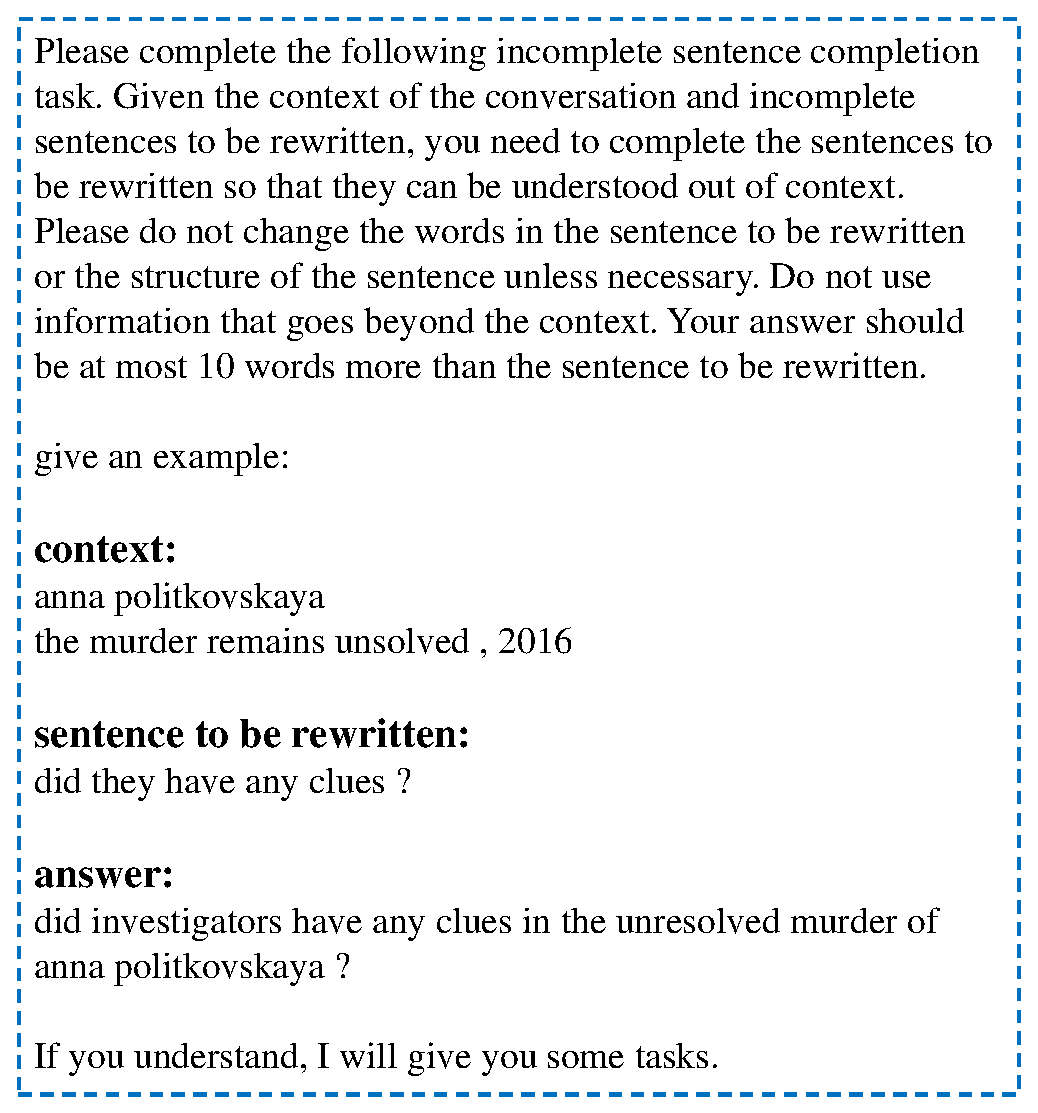
\includegraphics[width=1.0\columnwidth]{prompt.eps}
        \caption{A prompt designed to allow ChatGPT to do rewriting task.}
        \label{fig:prompt}
\end{figure}

The scale of ChatGPT or is at least 3 orders of magnitude larger than  the models we use in this paper, which means this is not a fair comparison. Nevertheless, we still conducted the following supplementary experiments on ChatGPT. The prompt we used is shown in \tabref{fig:prompt}.

\begin{table}[ht!]
%\setlength\tabcolsep{3pt}
\centering
\scriptsize
%\small
%\begin{tabular}{lrrrrrrr}
%\resizebox{\linewidth}{!}{
\begin{tabular}{l|ccc}
%\hline
\toprule
\textbf{Methods}&    \textbf{F}$_{1/2}$ & \textbf{BLEU}$_{1/2}$ & \textbf{ROUGE}$_{1/2/L}$  \\ \midrule
Ours-T5 & \textbf{46.6}/\textbf{33.3} & \textbf{63.5}/\textbf{53.9}  & \textbf{67.6}/\textbf{49.4}/\textbf{64.2}  \\ \midrule
ChatGPT &41.8/23.4  & 45.0/30.1 & 52.2/23.3/46.3  \\
\bottomrule
\end{tabular}
%}
\caption{Experimental results on 30 cases of CANARD.}
\label{tab:result-chatgpt}
\end{table}

The experimental results on 30 cases of CANARD is shown in \tabref{tab:result-chatgpt}. Some examples of the results are shown in \tabref{tab:excample-chatgpt}. After repeated tries and with the best prompt we can find, ChatGPT is still worse than our method in terms of automatic evaluation metrics. However, by human evaluation, testers think that the rewriting results of ChatGPT are of higher quality (more fluent). This is no surprise given the tremendous parameter space of ChatGPT.

\begin{table}[h]
\centering
\scriptsize
%\small
%\begin{tabular}{lrrrr}
\begin{tabular}{ll}
%\hline
\toprule
Ours-T5    & \tabincell{l}{did fsb get into trouble for the attack against the account\\
annapolitovskaya@us provider1 ? \\
why did superstar billy graham return to the wwwf ?} \\ \midrule
ChatGPT  & \tabincell{l}{Did the perpetrators face consequences for the attack\\
on Anna Politkovskaya's email? \\
What was the reason for Superstar Billy Graham's return \\
to WWWF?}\\
\bottomrule
\end{tabular}
\caption{Examples of ChatGPT and ours on CANARD.}
\label{tab:excample-chatgpt}
\end{table}